\chapter{Software Quality}

\section{Define aspects of software defects and defect management alternatives}

\textblue{Defect} = some problem with the software
\begin{itemize}
    \item[$\hookrightarrow$] (Human) Error : a mistake in performing some software activities
    \item[$\hookrightarrow$] Fault : a defect in the product
    \item[$\hookrightarrow$] Failure : a departure from the system's required behaviour
    \item[] \textblue{High quality} $\approx$ low defect
    \item[] \textblue{Quality problem} $\approx$ defect impact
\end{itemize}

\textblue{Dealing with defects :}

\begin{minipage}{0.48\textwidth}
\begin{enumerate}
        \item \textblue{Defect prevention} :
        \begin{itemize}
            \item [$\bullet$]Prevent faults from being injected
            \item [$\bullet$]Error blocking, error source removal
        \end{itemize}
        \item \textblue{Defect removal} :
        \begin{itemize}
            \item [$\bullet$]Remove faults
            \item [$\bullet$]Inspection (find faults), testing (find failures from faults
        \end{itemize}
        \item \textblue{Defect containment} :
        \begin{itemize}
            \item [$\bullet$]Keep failures local, reduce failure impact
            \item [$\bullet$]Fault-tolerance, failure containment
        \end{itemize}
    \end{enumerate}
\end{minipage}
\hfill
\begin{minipage}{0.48\textwidth}
    \begin{figure}[H]
        \centering
        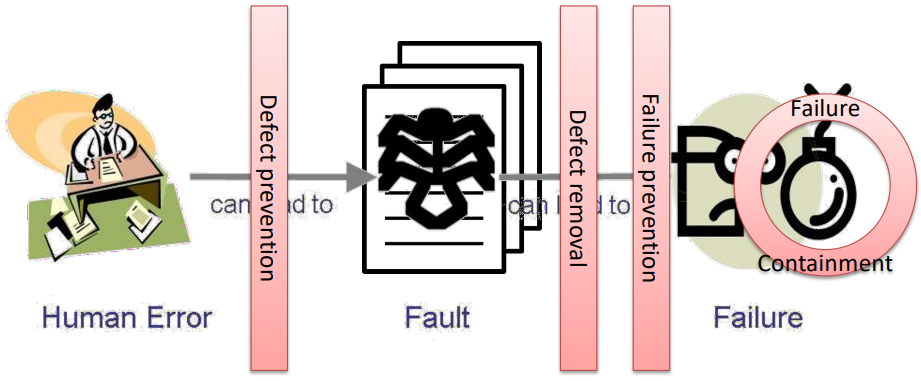
\includegraphics[width=\textwidth,keepaspectratio]{dealing_with_defects}
    \end{figure}
\end{minipage}

\section{Discuss different software quality characteristics and perspectives}

\textblue{What is good software ? What is quality ?}
\begin{itemize}
    \item \textit{Transcendental} view : an ideal that we thrive to but cannot attain
    \item \textit{User} view : fitness for purpose, reliability, absence of defects
    \item \textit{Manufacturing} view : conformance to the process
    \item \textit{Product} view : showing good inherent characteristics
    \item \textit{Value-based} view : how much the customer is willing to pay for it
\end{itemize}

Quality models relate the user's external view to the developer's internal view :

\begin{minipage}[t]{0.48\textwidth}
    \textblue{Consumers} $=$
    \begin{enumerate}
        \item \textblue{Client} : pay for the development
        \item \textblue{User} of software
        \item \textblue{Customers} : buy  after development
    \end{enumerate}
    Expect \textblue{external} qualities : 
    \begin{enumerate}
        \item good enough for the price
        \item fit‐for‐use, doing the right things
        \item conformance, doing things right
    \end{enumerate}
\end{minipage}
\hfill
\begin{minipage}[t]{0.48\textwidth}
    \textblue{Producers} $=$ Developer
    
    Expect \textblue{internal} qualities : 
    \begin{enumerate}
        \item good enough for the cost
        \item maintainable
        \item interoperable
        \item modular
    \end{enumerate}
\end{minipage}

\begin{minipage}[t]{0.48\textwidth}
    $\Rightarrow$ Judge \textblue{external} characteristics : number and type of \textblue{failures}
\end{minipage}
\hfill
\begin{minipage}[t]{0.48\textwidth}
    $\Rightarrow$ Judge \textblue{internal} characteristics : number and type of \textblue{faults}
\end{minipage}

\newpage
\section{Define correctness, reliability, safety and robustness}

These are "dependability properties" (Correctness properties are \textit{undecidable} for non-trivial programs): 
\begin{itemize}
    \item [$\bullet$]\textblue{Correctness:} a program is correct if it is consistent with its specification (seldom practical for non-trivial systems)
    \item [$\bullet$]\textblue{Reliability:} likelihood of correct function for some "unit" of behaviour, relative to a specification and usage profile, statistical approximation to correctness (100\% reliable = correct)
    \item [$\bullet$]\textblue{Safety:} preventing hazards, which are system-specific undesirable behaviours
    \item [$\bullet$]\textblue{Robustness:} acceptable (degraded) behaviour under extreme conditions
\end{itemize}

\begin{figure}[H]
    \centering
    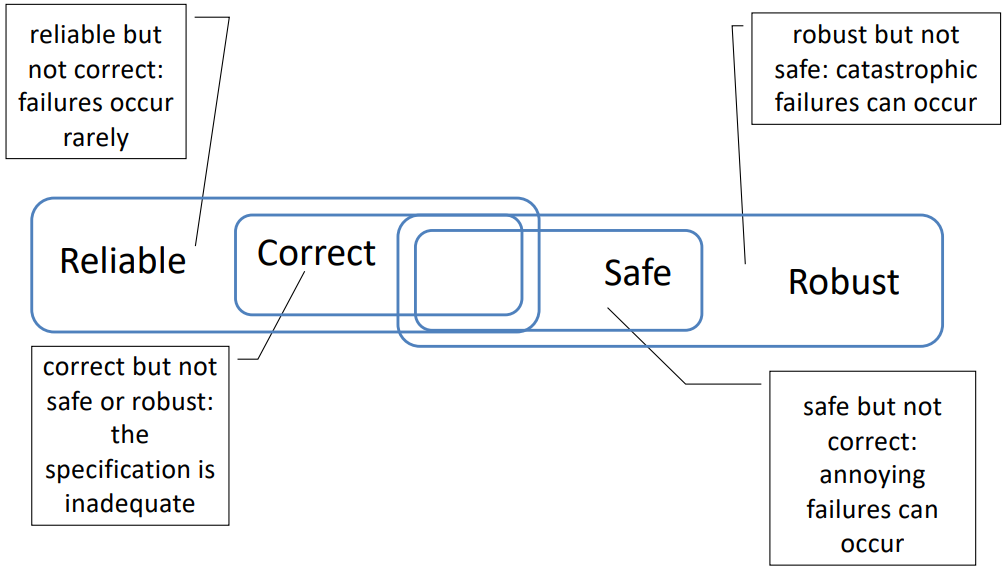
\includegraphics[width=0.7\textwidth,keepaspectratio]{realation_among_dq}
\end{figure}

\chapter{Software Development Process}

\section{Define software verification and validation}

\begin{minipage}[t]{0.48\textwidth}
    \textblue{Verification} $=$ does the software system meets the requirements specs ? Are we building the software right ?
    
    $\hookrightarrow$ Application conform to specifications
\end{minipage}
\hfill
\begin{minipage}[t]{0.48\textwidth}
    \textblue{Validation} $=$ does the software system meets the user's real need ? Are we building the right software ?
    
    $\hookrightarrow$ Specifications accurately reflects the customer's needs
\end{minipage}

\begin{minipage}[t]{0.48\textwidth}
    \textblue{Techniques} :
    \begin{enumerate}
        \item Consistency / Completeness / Reachability checks
        \item Model checking
        \item Mathematical proofs
    \end{enumerate}
\end{minipage}
\hfill
\begin{minipage}[t]{0.48\textwidth}
    \textblue{Techniques} :
    \begin{enumerate}
        \item Modelling
        \item Scenarios
        \item Prototypes
        \item Simulation
        \item[] ...
    \end{enumerate}
\end{minipage}

\section{Describe a software development process and how verification and validation activities fit into this process}

\textblue{Classic approach} : Requirement $\rightarrow$ Specifications $\rightarrow$ Design $\rightarrow$ Coding $\rightarrow$ Testing $\rightarrow$ Release

\textblue{Variation} : Waterfall, iterative, spiral, agile, ...

\begin{figure}[H]
    \centering
    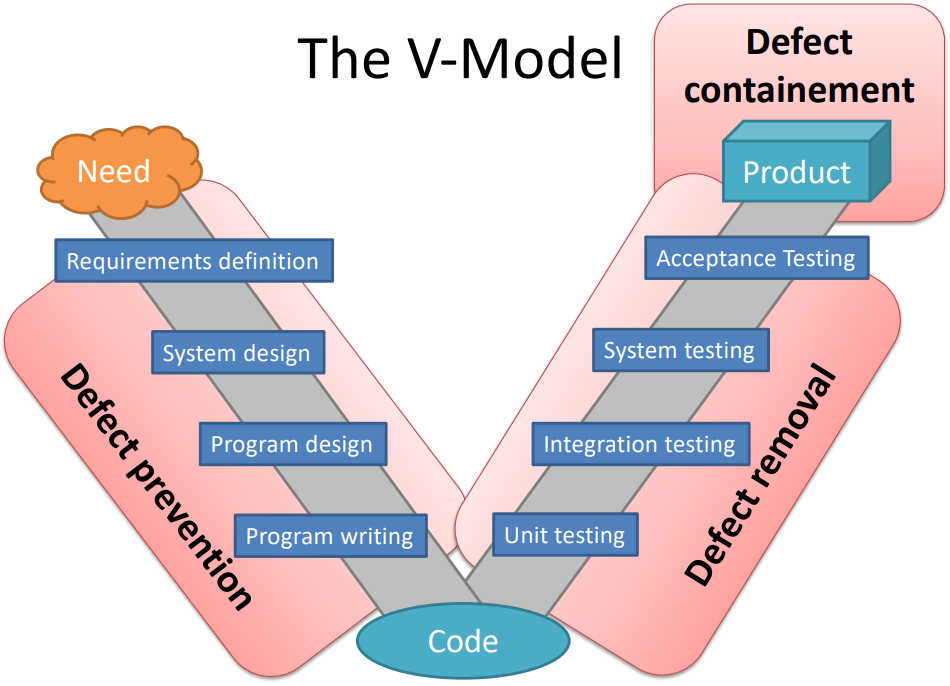
\includegraphics[width=0.48\textwidth,keepaspectratio]{v_model}\hfill
    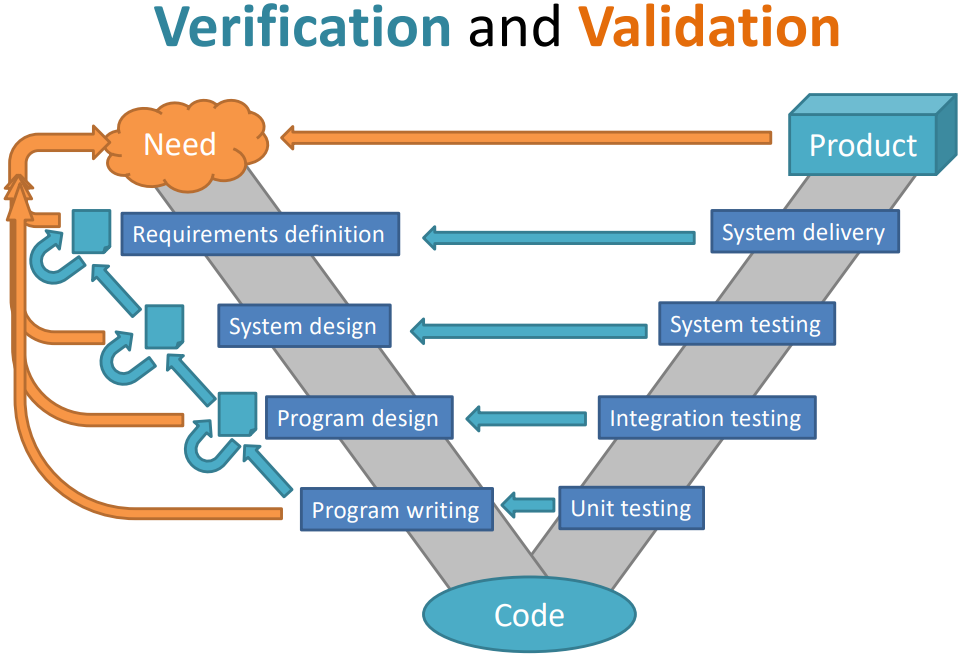
\includegraphics[width=0.48\textwidth,keepaspectratio]{v_v}
\end{figure}

\newpage
\section{Describe different types of software quality assurance activities}

\begin{enumerate}
    \item \textblue{Testing}
    \begin{itemize}
        \item Executing late in development
        \item Generate tests as early as possible
        \begin{itemize}
            \item Tests generated independently from code, when the specifications are fresh in the mind of analysts
            \item Generation of test cases may highlight inconsistencies and incompleteness of the corresponding specifications
            \item Tests may be used as compendium of the specifications by the programmers
        \end{itemize}
    \end{itemize}
    \item \textblue{Inspection}
    \begin{itemize}
        \item Can be applied to essentially any document (requirements statements, architectural and detailed design documents, test plans and test cases, program source code)
        \item May also have secondary benefits (spreading good practices, instilling shared standards of quality)
        \item Takes a considerable amount of time
        \item Re-inspecting a changed component can be expensive
        \item Used primarily where other techniques
         \begin{itemize}
            \item are inapplicable
            \item do not provide sufficient coverage
        \end{itemize}
    \end{itemize}
    \item \textblue{Automatic Static Analysis}
    \begin{itemize}
        \item More limited in applicability : can be applied to some formal representations of requirements models but not to natural language documents
        \item Are selected when available
        \begin{itemize}
            \item Substituting machine cycles for human effort makes them particularly cost-effective
        \end{itemize}
    \end{itemize}
        \item \textblue{Computer-Aided Verification}
    \begin{itemize}
        \item \textblue{Model checking} : exhaustive search of a specification's execution space
        \begin{itemize}
            \item Applicable to behaviour models (e.g. statecharts, Petri nets)
            \item Check state conditions, temporal logic, compare models
        \end{itemize}
        \item \textblue{Theorem proving} : prove Specifications AND Assumptions IMPLY Requirements
        \begin{itemize}
            \item Using built-in theories, inference rules, decision procedures
        \end{itemize}
    \end{itemize}
    \item \textblue{Improving the Process}
    \begin{itemize}
        \item Long lasting errors are common
        \item It is important to structure the process for
        \begin{itemize}
            \item the most critical persistent faults
            \item tracking them to frequent errors
            \item adjusting the development and quality processes to eliminate errors
        \end{itemize}
        \item Feedback mechanisms are the main ingredient of the quality process for identifying and removing errors
    \end{itemize}
\end{enumerate}

\chapter{Behaviour models}

\section{Define state models}

\textblue{Models} = \textit{abstraction} of the system (removes irrelevant attributes or details via an abstraction function)
\begin{itemize}
    \item Represent a system, an artefact, a design
    \item Analyse a system, an artefact, a design
    \begin{itemize}
        \item before the system is built
        \item easier to analyse/check/test than the actual system
    \end{itemize}
    \item \textblue{Properties} : Compact, Predictive, Semantically meaningful and Sufficiently general
\end{itemize}

\textblue{State models}
\begin{itemize}
    \item \textblue{Program execution} = sequence of states and transitions
    \begin{itemize}
        \item \textblue{States} : control + data (Location + variables, stack, heap)
        \item \textblue{Transitions} : actions (ops, instructions)
    \end{itemize}
    \item \textblue{State Space} :
    \begin{itemize}
        \item \textblue{Full} (all possible values)
        \item \textblue{Reachable} (from initial states)
    \end{itemize}
\end{itemize}

Essentially \textblue{infinite}
\textblue{Finite models} of program execution $\Rightarrow$ abstraction
\begin{enumerate}
    \item Execution is \textblue{coarsened} (fewer steps)
    \item \textblue{Nondeterminism} is introduced
\end{enumerate}

\section{Describe control flow graphs and their constituents}

\textblue{Abstraction} : set of program locations (PC) $\rightarrow$ finite number of locations

\textblue{Control Flow Graph (CFG)} :
\begin{itemize}
    \item \textblue{Nodes} = regions of source code (basics blocks)
    \begin{itemize}
        \item Basic block: maximal program region with a single entry and single exit point
        \begin{enumerate}
            \item Often several statements in one blocks
            \item Sometimes one statement in several blocks
        \end{enumerate}
    \end{itemize}
    \item \textblue{Edge} = possibility that execution proceeds from the end of one region to the beginning of another
\end{itemize}

\begin{figure}[H]
    \centering
    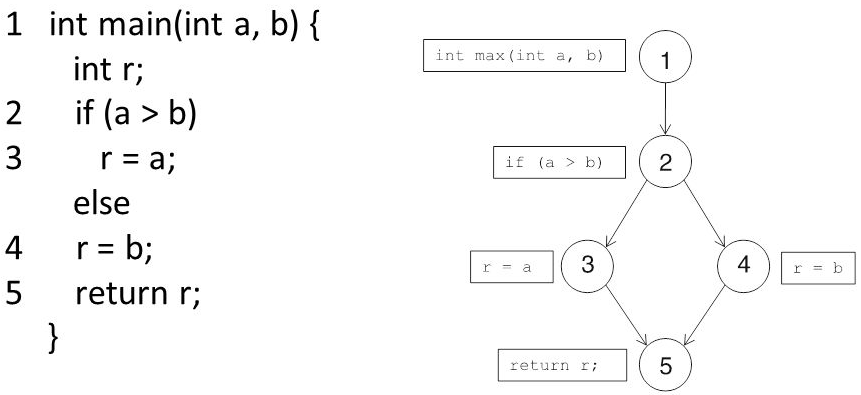
\includegraphics[width=0.65\textwidth,keepaspectratio]{cfg_example}
\end{figure}

$\Rightarrow$ \textblue{Intra-procedural} (ignore calls). May not cover some flows (e.g : exceptions are not covered)

\textblue{Linear Code Sequence and Jump (LCSJ)}: Subpaths from one branching point to another (jumps)

\section{Describe call graphs and discuss context-sensitive analysis}

\textblue{Call graphs} : 
\begin{itemize}
    \item Nodes represent procedures
    \item Edges represent calls relation
\end{itemize}

$\Rightarrow$ \textblue{Inter-procedural} 

\begin{figure}[H]
    \centering
    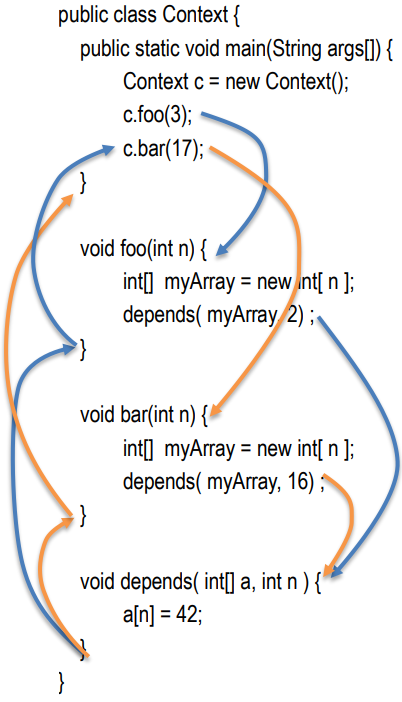
\includegraphics[width=0.23\textwidth,keepaspectratio]{call_graph_code}
\end{figure}

\begin{minipage}[t]{0.48\textwidth}
    Context-Insensitive Call Graph
    \begin{figure}[H]
        \centering
        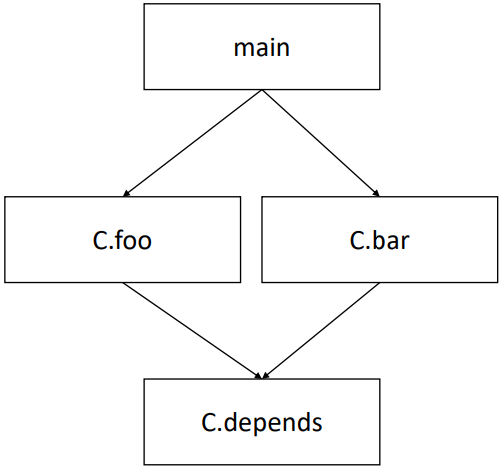
\includegraphics[width=0.6\textwidth,keepaspectratio]{call_graph_CI}
    \end{figure}
\end{minipage}
\hfill
\begin{minipage}[t]{0.48\textwidth}
    Context-Sensitive Call Graph
    \begin{figure}[H]
        \centering
        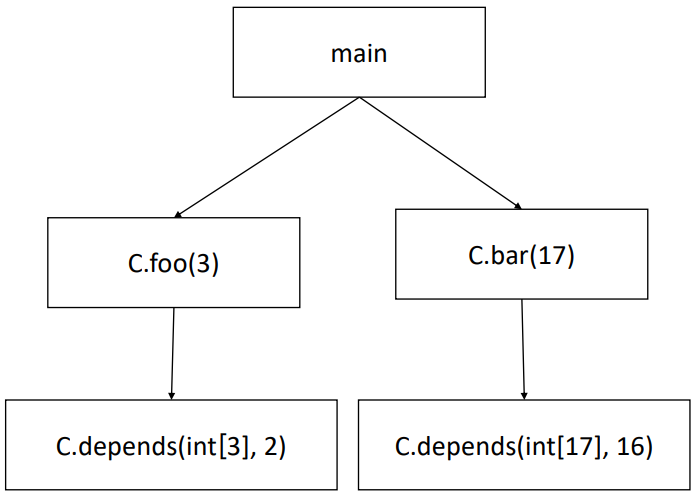
\includegraphics[width=0.8\textwidth,keepaspectratio]{call_graph_CS}
    \end{figure}
    Keep information about \textblue{calling context}, may infer that depends does not violate bounds of $a[...]$
\end{minipage}

\textblue{Context-sensitive analysis}:  the number of contexts grows exponentially with the depth of the calls :
\begin{itemize}
    \item $\#C \approx \#P^{depth}$
    \item Where $\#C$ is number of contexts and $\#P$ the number of procedures
\end{itemize}

\newpage
\section{Describe finite state machines and discuss abstraction}

\begin{itemize}
    \item  \textblue{Nodes} = states (finite number)
    \item  \textblue{Edges} = transitions
    \begin{itemize}
        \item Labelled with condition, operation, event
        \item Input/output : Mealy Machine
    \end{itemize}
    \item Used as \textblue{specifications} of allowed behaviour
\end{itemize}

For example, a transition diagram (Mealy machine) or a state-transition table.

\textblue{Abstraction function} : checking correctness with respect to the written program (Finite State Machine accurately represents program behaviour $\equiv$ program correctly implements FSM abstraction).

\textblue{Abstract} (function) : takes a program state returns a FSM state

\textblue{Example} :
\begin{figure}[H]
    \centering
    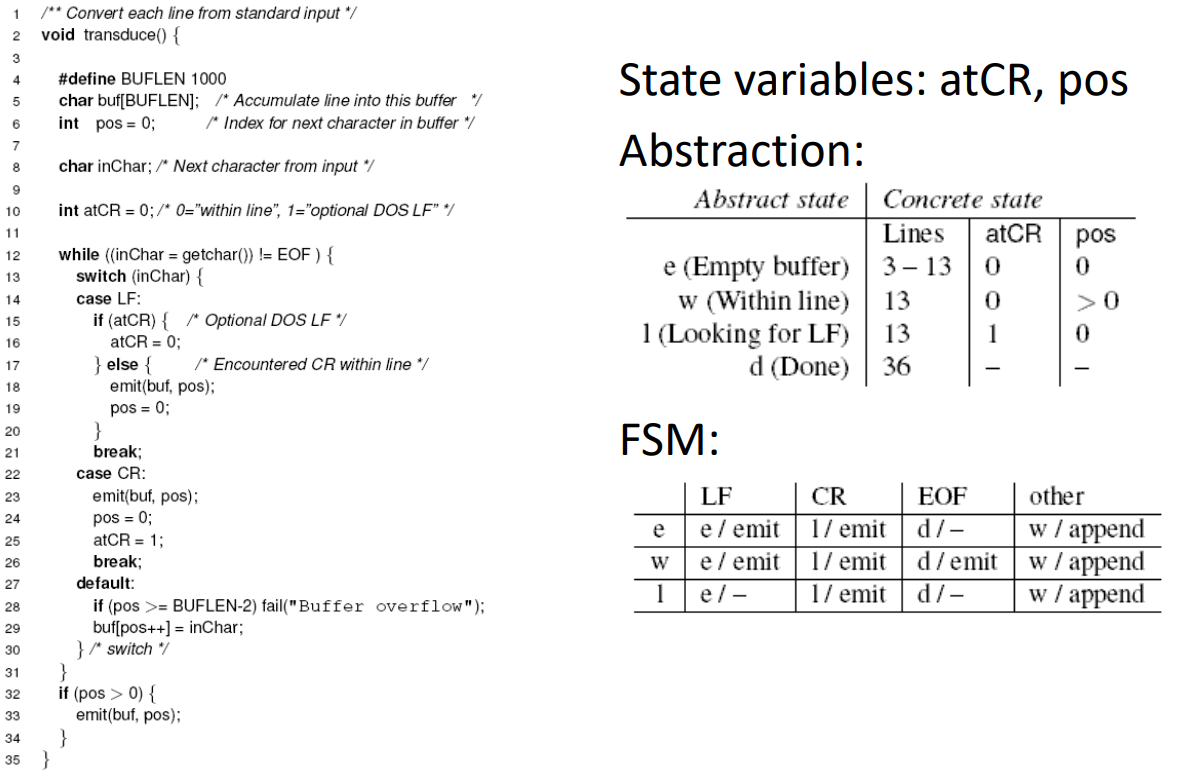
\includegraphics[width=\textwidth,keepaspectratio]{abstraction_example}
\end{figure}

\chapter{Data models}

\section{Define data dependence based on def-use pairs}

\begin{minipage}[t]{0.48\textwidth}
    \begin{enumerate}
        \item \textblue{Def} :

        Point where a variable gets a value (declaration, initialization, assignment or value received by parameter)
    \item \textblue{Use} :

    Point where a value from a variable is used (expression, conditional statement, parameter passing, returns)
    \item[$\Rightarrow$] \textblue{Def-Use pair} : Pair of points
    \begin{itemize}
        \item from where a value is produced
        \item to where that value is used
    \end{itemize}
\end{enumerate}
\end{minipage}
\hfill
\begin{minipage}[t]{0.48\textwidth}
\begin{figure}[H]
    \centering
    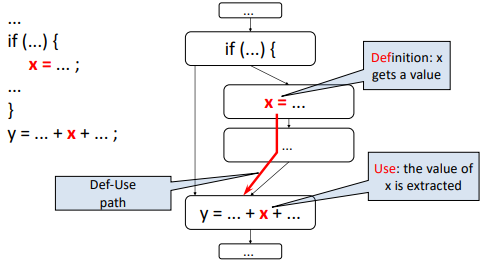
\includegraphics[width=\textwidth,keepaspectratio]{def_use}
\end{figure}
\end{minipage}

$\Rightarrow$ \textblue{Data dependence based on def-use pairs} : Where does this value of x come from? What would be affected by changing this? ...

\section{Describe data dependence and control dependence graphs}

\begin{minipage}[t]{0.48\textwidth}
    \textblue{Data dependence graph} :
    \begin{enumerate}
        \item \textblue{Nodes} :
        
        Program regions as in the control flow graph
        \item \textblue{Edges} :
        
        \textblue{Def-use pairs} labelled with the variable name
        \vspace{11pt}
        \item[$\Rightarrow$] \textblue{Data dependence} :
        
        P2 depends on P1 iff data values used in P2 can be defined in P1 (P1 is a         \textblue{definition point}, P2 is an \textblue{use point})
    \end{enumerate}
\end{minipage}
\hfill
\begin{minipage}[t]{0.48\textwidth}
    \textblue{Control dependence graph} :
    \begin{enumerate}
        \item \textblue{Nodes} :
        
        Program regions as in the control flow graph
        \item \textblue{Edges} :
        
        From \textblue{entry / branching} points to controlled blocks
        \item[$\Rightarrow$] \textblue{Control dependence} :
        
        P2 depends on P1 iff P1 controls whether P2 executes (P1 is an \textblue{entry / branching point}, P2 is \textblue{any point})
    \end{enumerate}
\end{minipage}

\begin{minipage}{0.48\textwidth}
    \begin{figure}[H]
        \centering
        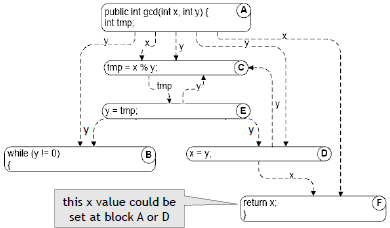
\includegraphics[width=\textwidth,keepaspectratio]{data_dep_g}
    \end{figure}
\end{minipage}
\hfill
\begin{minipage}{0.48\textwidth}
    \begin{figure}[H]
        \centering
        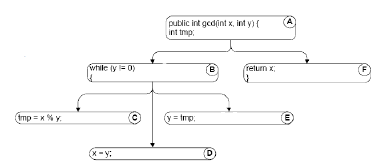
\includegraphics[width=\textwidth,keepaspectratio]{control_dep_g}
    \end{figure}
\end{minipage}

The difference with control flow is that blocks of CFG only follow other blocks but do not depends on them. Either of these blocks could be executed in either order.

\newpage
\section{Explain the general principle of dataflow analyses based on worklist algorithms, and the particular case of computing reaching definitions}

\textblue{Reaching definition}

\begin{minipage}{0.64\textwidth}
    Let :
    \begin{enumerate}
        \item $v_d, v_e$ definitions of variables $v$ at points $d,e$
        \item $u$ a point where $v$ is used
        \item[$\Rightarrow$] Definition $v_d$ \textblue{reaches} $u$ ($v_d$ is a \textblue{reaching definition} at $u$) iff 
        \begin{enumerate}
            \item There is at least one control flow path from $d$ to $u$
            \item There is no intervening definition of $v$ on the path
        \end{enumerate}
        \item[$\Rightarrow$] $v_e$ \textblue{kills} $v_d$ iff it is on a control path from $d$
        \item[$\Rightarrow$] $(d,u)$ is a \textblue{def-use pair} of $v$ iff $v_d$ \textblue{reaches} $u$
    \end{enumerate}
\end{minipage}
\hfill
\begin{minipage}{0.35\textwidth}
    \begin{figure}[H]
        \centering
        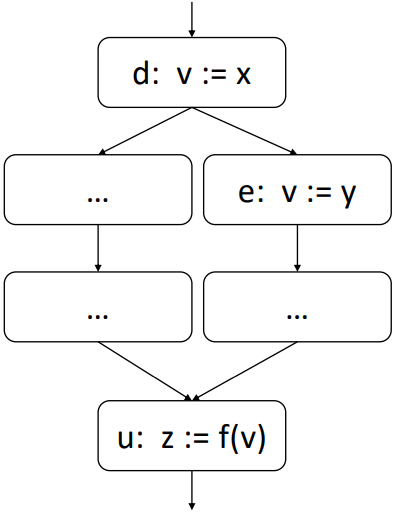
\includegraphics[width=0.5\textwidth,keepaspectratio]{reaching_def}
    \end{figure}
\end{minipage}

\textblue{Calculating Def‐Use Pairs}

Even with loop‐free paths, the number of paths in a graph can be \textblue{exponentially larger} than the number of nodes and edges. So we don’t want to search every individual path but we want to summarize the reaching definitions at a node over all the paths reaching that node.

\textblue{DF Algorithm} :

\begin{itemize}
    \item \textblue{Goal} : compute reaching definitions at node $n$
    \item Suppose that node $p$ is an immediate predecessor of node $n$
    \begin{itemize}
    \item If $p$ can assign variable $v$, then $v_p$ reaches $n$. We say the definition $v_p$ is generated at $p$
    \item If a definition $v_d$ reaches $p$, and if $v$ is not redefined at $p$, then $v_d$ reaches $n$.
    \end{itemize}
    \item $Reach(n) =$ set of definitions that reach $n$
    \item $ReachOut(n) =$ set of definitions that exit $n$
\end{itemize}
\begin{figure}[H]
    \centering
    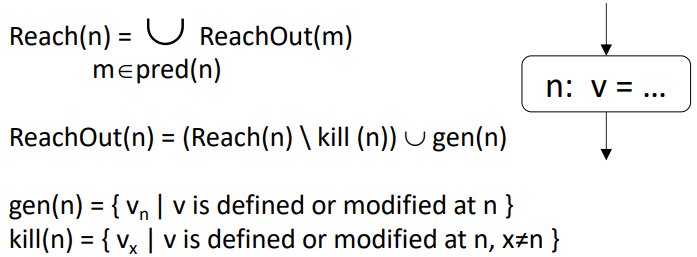
\includegraphics[width=0.5\textwidth,keepaspectratio]{reach_analysis}
\end{figure}
\begin{itemize}
    \item[$\Rightarrow$] \textblue{Recursive equations} for all nodes $n$
    \item[$\Rightarrow$] \textblue{Fixed point} computation
\end{itemize}

\textbf{Worklist Algorithm} :
\begin{figure}[H]
    \centering
    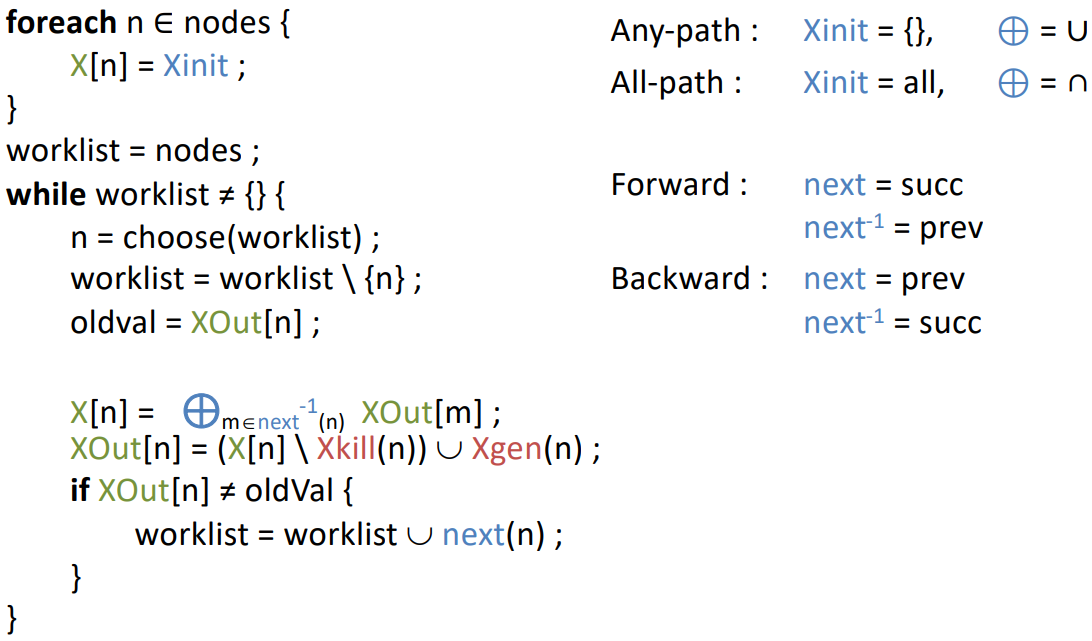
\includegraphics[width=0.7\textwidth,keepaspectratio]{worklist_alg}
\end{figure}

\textbf{Example} :
\begin{figure}[H]
    \centering
    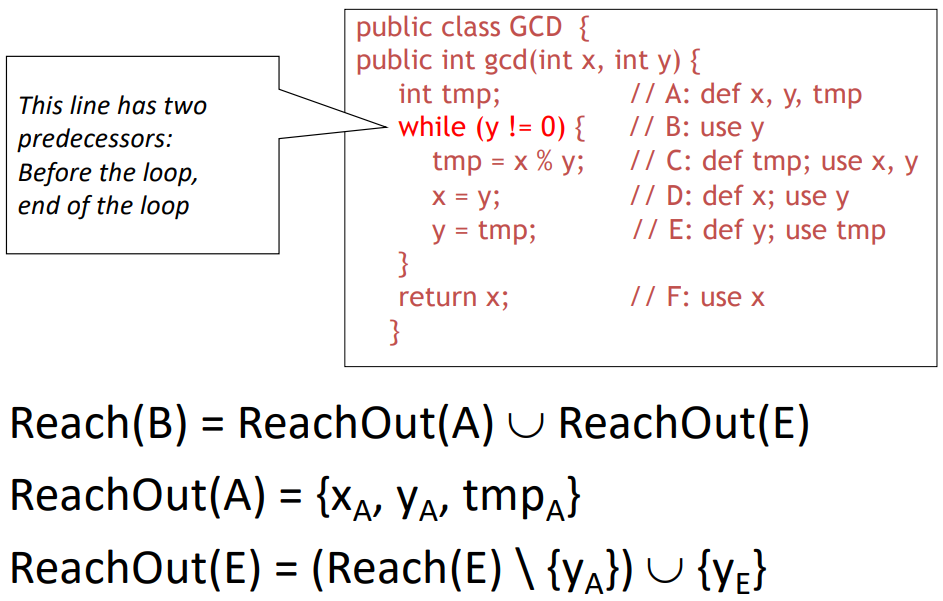
\includegraphics[width=0.6\textwidth,keepaspectratio]{worklist_ex_1}\\
    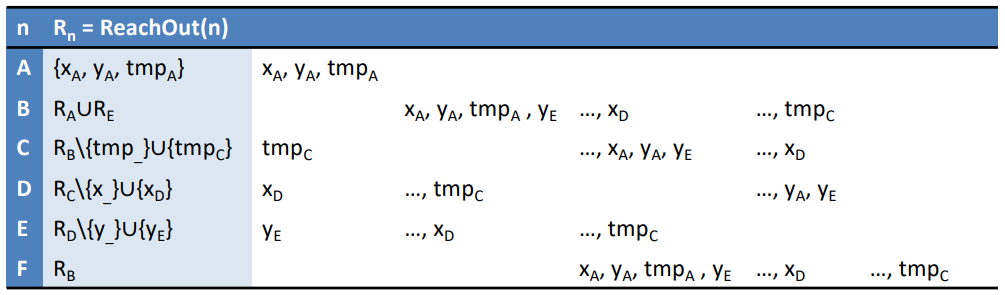
\includegraphics[width=0.7\textwidth,keepaspectratio]{worklist_ex_2}
\end{figure}

\textbf{Particular cases} :
\begin{enumerate}
    \item \textblue{Avail expressions} : expression $exp$ is \textblue{available} at node $n$ iff for all paths to $n$, $exp$ has been computed and not subsequently modified (used in compiler construction)
    \begin{figure}[H]
        \centering
        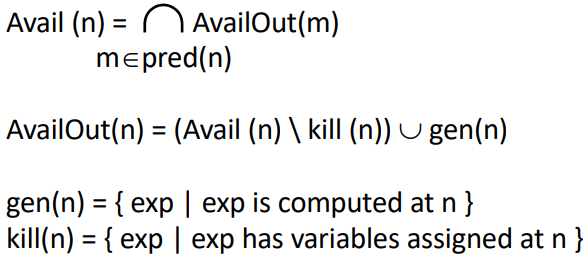
\includegraphics[width=0.4\textwidth,keepaspectratio]{avail_exp}
    \end{figure}
    \item \textblue{Live variables} : A variable $v$ is \textblue{live} at node $n$ iff on some execution path from $n$, $v$ is used before it is changed
    \begin{figure}[H]
        \centering
        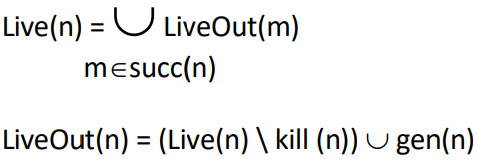
\includegraphics[width=0.4\textwidth,keepaspectratio]{live_exp}
    \end{figure}
\end{enumerate}

\textbf{Classification of analyses} :
\begin{itemize}
    \item \textblue{Forward/backward} : a node’s set depends on that of its predecessors/successors
    \item \textblue{Any-path/all‐path} : a node’s set contains a value iff it is coming from any/all of its inputs
\end{itemize}

\begin{figure}[H]
    \centering
    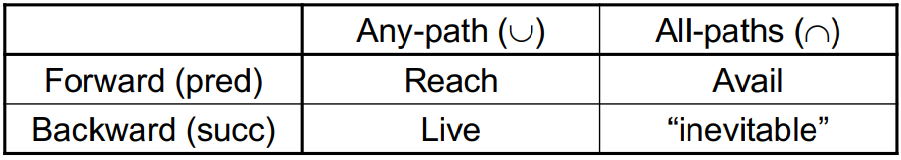
\includegraphics[width=0.5\textwidth,keepaspectratio]{classification_of_analyses}
\end{figure}

\section{Discuss the effect of pointers and procedures.}

\begin{enumerate}
    \item \textblue{Arrays and pointers} : introduce \textblue{uncertainty} : do different expressions access the same storage ?
    
    For example: $a[i]$ is the same as $a[k]$ when $i=k$ or $a[i]$ same as $b[i]$ when $a=b$. 
    
    \textblue{Solution}: 
    \begin{enumerate}
        \item \textblue{Any-path} : Gen sets contains all potential aliases, kill sets contain only what is definitely modified.
        \item \textblue{All-path} : Vice versa
    \end{enumerate}
    \item \textblue{Procedures} : \textblue{interprocedural} (Across several methods or procedures) data flow analysis has critical and difficult cost/precision trade-offs: context sensitivity and flow sensitivity.
    
    For example: Reach, Avail,... are flow-sensitive and \textblue{intraprocedural} (Within a single method or procedure) analyses which cost \bigO$(n^3)$ for one procedure (reasonably cheap) but what about doing flow-sensitive interprocedural analyses? $\rightarrow$ \bigO$(n^3)$ on the whole program : prohibitive ! So, many interprocedural flow analyses are flow-insensitive (it is often good enough, e.g. type checking)
\end{enumerate}

\chapter{Functional testing}

\section{Define test case, test obligation, adequacy criterion, test satisfaction}

\begin{enumerate}
    \item \textblue{Test case} : A set of inputs, execution conditions, and a pass/fail criterion for judging test execution
    \item \textblue{Test case specification} : A requirement to be satisfied by one or more test cases
    \item \textblue{Test obligation} : A partial test case specification, requiring some property deemed (= considered) important to thorough testing
    \item \textblue{Adequacy criterion}: A predicate that a <program, test suite> pair must satisfy; usually expressed in the form of a rule for deriving a set of test obligations from another artefact (program, specification)
    \item \textblue{Test satisfaction}:
    A test suite (set of test cases) satisfies an adequacy criterion if :
    \begin{itemize}
        \item All the tests succeed (pass)
        \item Every obligation is satisfied by at least one test case
    \end{itemize}
\end{enumerate}

\textblue{Infeasible Criterion}: Sometimes no test suite can satisfy a criterion for a given program
\begin{itemize}
    \item [$\Rightarrow$] Solution : eliminate infeasible test obligations\\
    $\hookrightarrow$ Undecidable in the general case
    \item [$\Rightarrow$] \textblue{Solution}: measure fraction of obligations covered\\
    $\hookrightarrow$ Coverage = \% of obligations covered
\end{itemize}

\section{Define functional and structural testing}

\begin{enumerate}
    \item \textblue{Functional testing} : (black box, closed box)
    \begin{itemize}
        \item Program content is unknown or ignored
        \item Test input/output behaviour
        \item Obligations from functional specifications (informal textual specs, tables, state graphs, UML, ...)
        \item [$\hookrightarrow$] Functional testing is \textblue{systematic testing} (select inputs that are especially valuable, different classes, limit cases, special values)
    \end{itemize}
    \item \textblue{Structural testing} : (white box, clear box)
    \begin{itemize}
         \item Program content is visible and observed (e.g. if test suite executes all program statements/conditions/branches/..., then coverage is 100\%)
         \item Test internal operation
         \item Obligations from program code
     \end{itemize}
\end{enumerate}

\newpage
\section{Explain category-partition testing}

\textblue{Category-partition testing} : 3 steps
\begin{enumerate}
    \item \textblue{Decompose the specification into units, parameters, categories}
    \begin{enumerate}
        \item Identify independently testable units
        \item For each unit, identify parameters and environment elements
        \item For each parameter, identify categories (characteristics) $\rightarrow$ Not a trivial task ! No hard-and-fast rules, reflect test designer’s judgment,...
    \end{enumerate}
    \item \textblue{Identify relevant choices (values) for each category}
    \begin{enumerate}
        \item Identify classes of values for each category (ignore interactions
between different categories)

        \item Boundary value testing
        \begin{enumerate}
            \item extreme values within a class
            \item values just outside the class
            \item interior (non-extreme) values
        \end{enumerate}
        \item Erroneous condition testing : values outside the normal domain of the program
    \end{enumerate}
    \item  \textblue{Introduce constraints} : combination of values for each category corresponds to a test case specification. Number of combinations = product of category sizes, most of which are impossible ! Introduce constraints to rule out impossible combinations, or to reduce the size of the test suite if too large
\end{enumerate}

\section{Explain pairwise and n-wise testing}

Category-partition testing is a systematic approach to generate combinations, but the test suite size grows very rapidly with the number of categories (even with constraints). The idea of pairwise testing is to use a non-exhaustive approach

\begin{enumerate}
    \item \textblue{Pair-wise testing} : all \textblue{pairs of choices}
    \begin{itemize}
        \item \textblue{Pairwise combination} : generate combinations that efficiently cover all pairs (triples,... in case of n-wise) of choices. Justified by the fact that most failures are triggered by a single value or a combination of a few values, so covering pairs (triples,...) reduces the number of test cases, but reveals most faults
        \item \textblue{Complexity} : For N categories with M choices each :
        \begin{itemize}
            \item \textblue{All combinations} $=$ \bigO$(M^N)$ test cases $\rightarrow$ exponential in number of categories
            \item \textblue{All pairs} $=$ \bigO$(M^2  log(N))$ test cases $\rightarrow$ logarithmic in number of categories
        \end{itemize}
    \end{itemize}
    \item \textblue{N-wise testing} : Same as pairwise but for all N-tuples of choices
\end{enumerate}

\newpage
\section{Explain catalog-based testing}

\begin{itemize}
    \item Deriving value classes requires human judgment, catalog-based testing aims to gather experience in a systematic collection
    \item Catalogs list important cases for each possible type of variable
\end{itemize}

\textblue{Benefits} :
\begin{itemize}
    \item Speed up the test design process
    \item Routinise many decisions, better focusing human effort
    \item Accelerate training and reduce human error
\end{itemize}

\textblue{Process} :
\begin{enumerate}
    \item Analyse the initial specification to identify simple
elements : pre-conditions, post-conditions, definitions,
variables, operations
    \item Derive a first set of test case specifications from pre-conditions, post-conditions
and definitions
    \item Complete the set of test case specifications using test catalogs
\end{enumerate}


\textblue{Catalog} :

\begin{itemize}
    \item Each entry $=$ a kind of element that can occur in a specification
    \item Each entry is associated with a list of generic test case specifications
\end{itemize}

\textblue{Example} :

\begin{itemize}
    \item Catalog entry Boolean
    \item Two test case specifications : $true, false$
    \item Label in/out indicate if applicable only to $input/output$ or $both$
\end{itemize}

\begin{figure}[H]
    \centering
    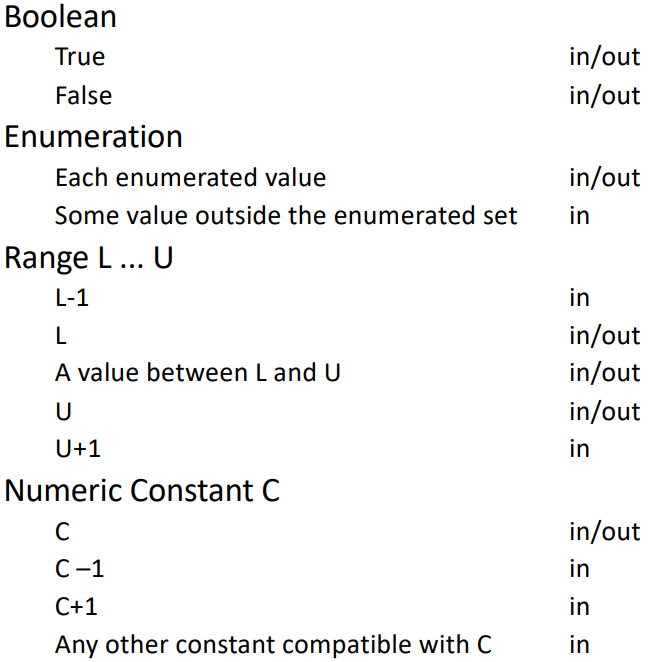
\includegraphics[width=0.5\textwidth,keepaspectratio]{catalog_ex}
\end{figure}

\chapter{Structural testing}

\chapter{Model-based testing}

\chapter{Object-oriented testing}

\chapter{Fault-based testing}

\chapter{Test execution I}

\chapter{Test execution II}

\chapter{Symbolic execution}

\chapter{Program analysis}

\chapter{Finite state analysis I}

\chapter{Finite state analysis II}

\chapter{Software measurement: size}

\chapter{Software measurement: structure}

\chapter{Software measurement: quality}

\chapter{Software reliability}

\chapter{Failure prediction}

